\section{Background}
\subsection{Embedded systems}
\justify
The definition of embedded systems varies among people. Some people, who 
work with desktop application or web application, may refer mobile devices 
as an embedded system. Some, however, who has developed application for 
8-bit microcontroller system seem not to agree. Though it is hard to define, 
embedded systems share some common characteristics:
\begin{itemize}
    \item Application-specific: 
        As opposed to general purpose computing device such as personal 
        computer, embedded devices are developed with pre-defined use cases 
        in mind and only offer a limited set of functions.
    \item Real world interaction:
        Embedded systems are developed to solve real world problem. They can
        be used to control some hardware, sense the environment with sensors, 
        or manipulate the physical world with actuators.  
    \item Constraints of hardware: 
        The resources, such as energy, CPU, memory, are limited. There are
        several ways to classify hardware used in embedded systems in terms 
        of resources. For instance, the Internet Engineering Task Force has 
        its own taxonomy of constrained-node networks \cite{BEK14}: 
        \begin{itemize}
            \item Class 0 devices have smallest resources, typically 
                $\ll$ 10 KiB of RAM and $\ll$ 100 KiB of Flash size.
            \item Class 1 devices have medium-level resources, typically 
                $\sim$ 10 KiB of RAM and $\sim$ 100 KiB of Flash size.
            \item Class 2 devices have more resources, typically 
                $\sim$ 50 KiB of RAM and $\sim$ 250 KiB of Flash size. 
        \end{itemize}
    \item Constraints of software: 
        Some systems require the software must act deterministically, soft 
        real-time, or hard real-time. Other systems require that the software
        be fault-tolerant in the face of errors (e.g., flight control systems
        on airplane) or to cease the operation at the first sign of problem (e.g.,
        medical devices). \cite[~1]{White11} 
\end{itemize}
An example of an embedded device is shown in figure 1, an IoT sensor kit named
Nordic Thingy:52. This is an easy-to-use protyping platform helping in rapidly
building prototypes and demos \cite{Thingy19}. 
\begin{figure}[H]
\centering
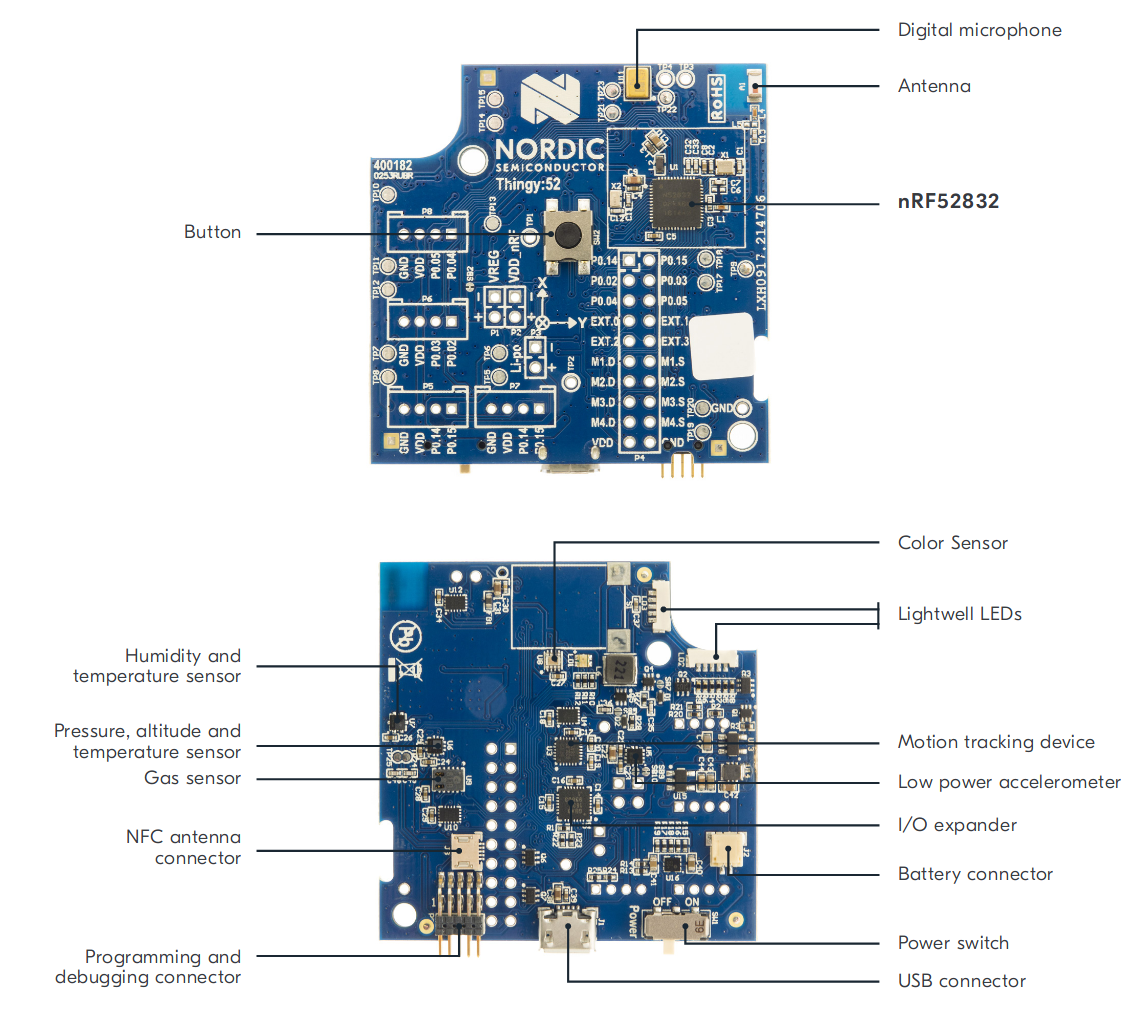
\includegraphics[scale=1.6]{figure/figure01_thingy_52.png}
\caption{Nordic Thingy:52. Adapted from \cite{Thingy19}.}
\end{figure}
\justify
As illustrated in figure 1, Nordic Thingy:52 consists of several components of an
typical embedded system:
\begin{itemize}
    \item Microcontroller/Microprocessor/System-on-Chip (SoC): 
        This is the heart of the system as it glues all components together.
        Its key job is to communicate with sensors for input variables and 
        actuators for output variables as well as processing the data. Other 
        hardware are built into the chip to assist these communication such as 
        analog-to-digital converter, digital-to-analog converter, and so on.

    \item Sensors:
        Each application interests to different set of data for its purposes. 
        The data collected by these sensors serve as the input to the system.
        The example device includes different types of sensors, such as color
        sensor, humidity and temperature sensor, and others.
    \item Actuators:
        In order to manipulate the environment in which the device operates,
        some actuators has to be built into the system. After processing the 
        input data collected by sensors, the cetral controller outputs signal 
        to control some actuators, for instance, LEDs, screen, to perform 
        the desired actions.    
    \item Power supply:
        This is the essential component of the system. Two primary sources of 
        power supply for an embedded system are wall power and batteries. Hence,
        the system could be powered by any one of these models:
        \begin{itemize}
            \item Wall powered
            \item Wall powered with battery as a backup
            \item Battery powered
        \end{itemize}
    \item Interfaces with other systems:
        An embedded system usually has some interfaces to communicate with other
        systems. They can be, for example, programming and debugging interface, 
        or USB port. They are important part of the system not only to the developer,
        who have to use debugging interface to aid the development process, but also
        the user to extend the existing functionalities by incorporating other devices.  
    \item Other application-specific components:
        Some systems require specific components for their application. For example, 
        the nRF52832 SoC needs an external antenna for wireless communication.
\end{itemize}

\subsection{Bluetooth Low Energy}

\subsection{Project overview}

\subsection{Hardware overview}